\documentclass[xcolor=dvipsnames, 14pt]{beamer}
%\documentclass[xcolor=dvipsnames, bigger, aspectratio=169]{beamer}

\definecolor{Saffron}{HTML}{F4C430}
\usecolortheme[named=Saffron]{structure}

\mode<presentation> {
	\usetheme[height=2em]{Rochester}
	\setbeamercovered{transparent}
}

\setbeamertemplate{caption}{\insertcaption\par}
\setbeamertemplate{navigation symbols}{}%remove navigation symbols

\setbeamercolor{frametitle}{fg=black}
\setbeamercolor{title}{fg=black}
\setbeamercolor{navigation symbols dimmed}{fg=black!10}
\setbeamercolor{navigation symbols}{fg=black!30}
\setbeamercolor{section number projected}{fg=black}
\setbeamercolor{item projected}{fg=black}


\usepackage[utf8x]{inputenc}
\usepackage[resetfonts]{cmap}
\usepackage{lmodern}
\usepackage[english]{babel}
\usepackage[T1]{fontenc}

\usepackage{graphicx}
\usepackage{amsmath}
\usepackage{amssymb}
\usepackage{listings}
\usepackage{microtype}
\usepackage{tikz}

\usepackage{hyperref}
\hypersetup{unicode=true}

% ----- macros -----
\newcommand{\imageW}[1]{%
  \makebox[\textwidth][c]{\includegraphics[width=1.12\textwidth]{img/#1}}}
\newcommand{\imageH}[1]{%
  \makebox[\textwidth][c]{\includegraphics[height=1.0\textheight]{img/#1}}}

% ---- info -----
\title{Adaptive Programming}
\author{Jaroslav~Čechák \and Tomáš~Effenberger \and  Jiří~Mauritz \and Jakub Peschel}
\institute{Faculty of Informatics, Masaryk University}
\date{\today}

\begin{document}

\begin{frame}
\titlepage
\end{frame}

\begin{frame}
\frametitle{Goal}
\begin{itemize}
\item application for learning programming efficiently
  \begin{itemize}
  \item teaching useful skills
  \item engaging tasks of optimal difficulty
  \item state of flow $\rightarrow$ learning maximized
  \end{itemize}
\item short term (this course): first prototype
\end{itemize}
\end{frame}

\begin{frame}
\frametitle{Flow}
\begin{figure}[h]
  \centering
  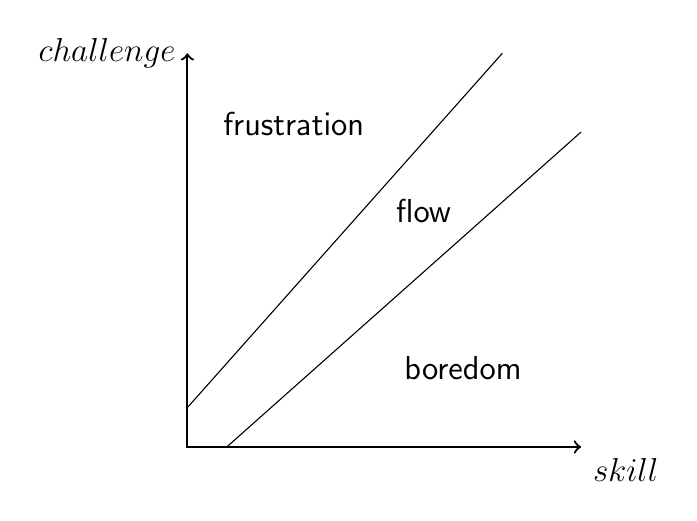
\begin{tikzpicture}[font=\sffamily,xscale=5, yscale=5]
  \large
  %\draw [lightgray, fill=gray] (0,0) -- (0.1,0) -- (1,0.8) -- (0.8,1) -- (0,0.1) -- (0,0);
  \draw (0.1,0) -- (1,0.8);
  \draw (0,0.1) -- (0.8,1);
  \draw [thick, <->] (0,1) node [left] {$challenge$} -- (0,0) -- (1,0) node [below right] {$skill$};
  \node at (0.27,0.82) {frustration};
  \node at (0.6,0.6) {flow};
  \node at (0.7,0.2) {boredom};
  \end{tikzpicture}
  %\caption{Relationship between challenge and skill.}
\end{figure}
\end{frame}

\begin{frame}
\frametitle{Existing projects and research}
\begin{itemize}
\item many websites for learning programming
  \begin{itemize}
  \item code.org, codecademy.com, Khan Academy, \ldots
  \item great in motivation, but no adaptivity
  \end{itemize}
\item engagement: robot in a grid, (turtle) graphics
\item avoiding syntax problems (Blockly, Scratch)
\item research: ITS (outer/inner loop, hints)
\item Problem Solving Tutor -- using time %-- skills and difficulties estimation
\end{itemize}
\end{frame}

\begin{frame}
\frametitle{Developed prototype}
\imageW{easy-task-initial.png}
\end{frame}

\begin{frame}
\frametitle{Developed prototype}
\imageW{easy-task-program.png}
\end{frame}

\begin{frame}
\frametitle{Developed prototype}
\imageW{easy-task-solved.png}
\end{frame}

\begin{frame}
\frametitle{Developed prototype}
\imageW{task-loops-initial.png}
\end{frame}

\begin{frame}
\frametitle{Developed prototype}
\imageW{complex-program.png}
\end{frame}

\begin{frame}
\frametitle{Developed prototype}
\imageW{task-colors.png}
\end{frame}

\begin{frame}
\frametitle{Developed prototype}
\imageW{task-keys.png}
\end{frame}

\begin{frame}
\frametitle{Developed prototype}
\imageW{task-pits.png}
\end{frame}

\begin{frame}
\frametitle{Model}
\begin{itemize}
\item skill, difficulties (biases, factors)
\item online parameters estimation
  \begin{itemize}
  \item collaborative filtering -- Elo model
  \item learning
  \end{itemize}
\item initial parameters values
  \begin{itemize}
  \item low initial skill
  \item content based approach for difficulties
  \end{itemize}
\end{itemize}
\end{frame}

\begin{frame}
\frametitle{Notation}
\begin{itemize}
\item $s$ -- student, $t$ -- task
\item $f_{st}$ -- reported flow
  \begin{itemize}
  \item -1 = too difficult
  \item 0 = just right
  \item 1 = too easy
  \end{itemize}
\item $\hat{f}_{st}$ -- predicted flow
\item $\beta_s, \alpha_s$ -- skill bias, skill factors vector
\item $b_s, a_s$ -- difficulty, difficulty factors vector
\end{itemize}
\end{frame}

\begin{frame}
\frametitle{Factors}
\begin{itemize}
\item concept factors
  \begin{itemize}
  \item loops
  \item conditions
  \item logic expressions
  \end{itemize}
\item game factors
  \begin{itemize}
  \item colors
  \item tokens
  \item pits
  \end{itemize}
\end{itemize}
\end{frame}

\begin{frame}
\frametitle{Factors}
\centering
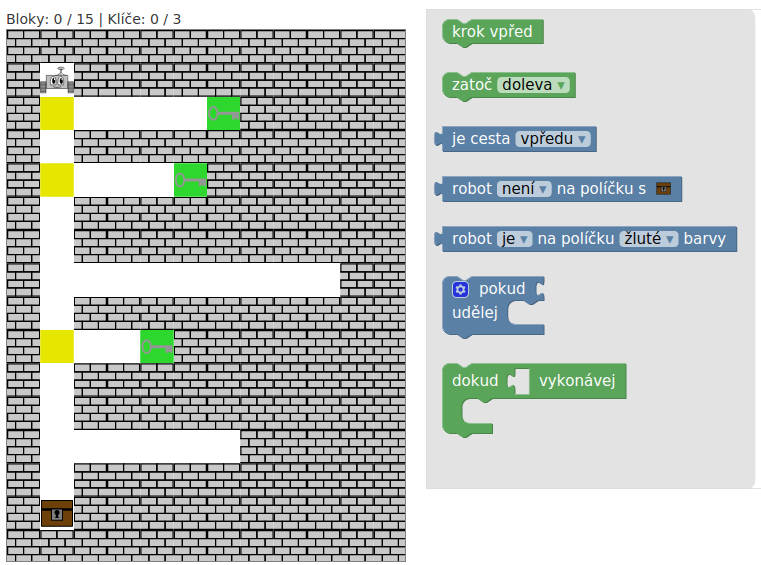
\includegraphics[height=6.3cm]{img/task-colors-keys-loops-conditions.png}
\[
  a_t = (0.2, 0.2, 0, 0.2, 0.2, 0)
\]
\end{frame}

\begin{frame}
\frametitle{Flow prediction}

\begin{block}{Predicted flow}
\[
  \hat{f}_{st} = \sigma ( \beta_s - b_t + \alpha_s \cdot a_t )
\]
\end{block}

where $\sigma (x) = K_{am} \tanh (K_{st} \cdot x)$,
$K_{am} = 1.7$, $K_{st} = \frac{2}{3}$

\centering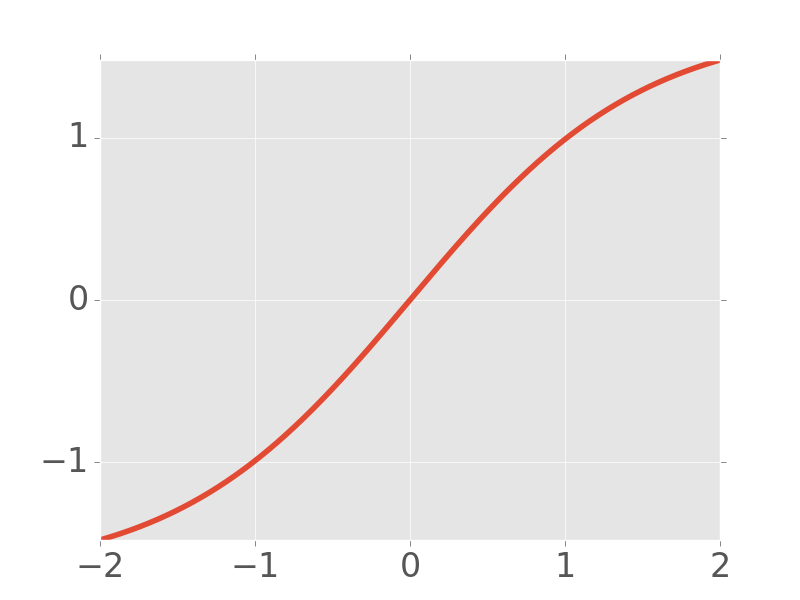
\includegraphics[height=4cm]{img/tanh.png}
\end{frame}

\begin{frame}
\frametitle{Task selection}
\begin{itemize}
\item criteria: flow prediction, time since last attempt
\item select task which maximizes scoring formula
\item $score(s, t) = W_F S_F(t, f) + W_T S_T(t, f)$
\item $W_F, W_T$ -- weights for flow and time
\item $S_F, S_T$ -- partial scores for flow and time
\end{itemize}
\centering
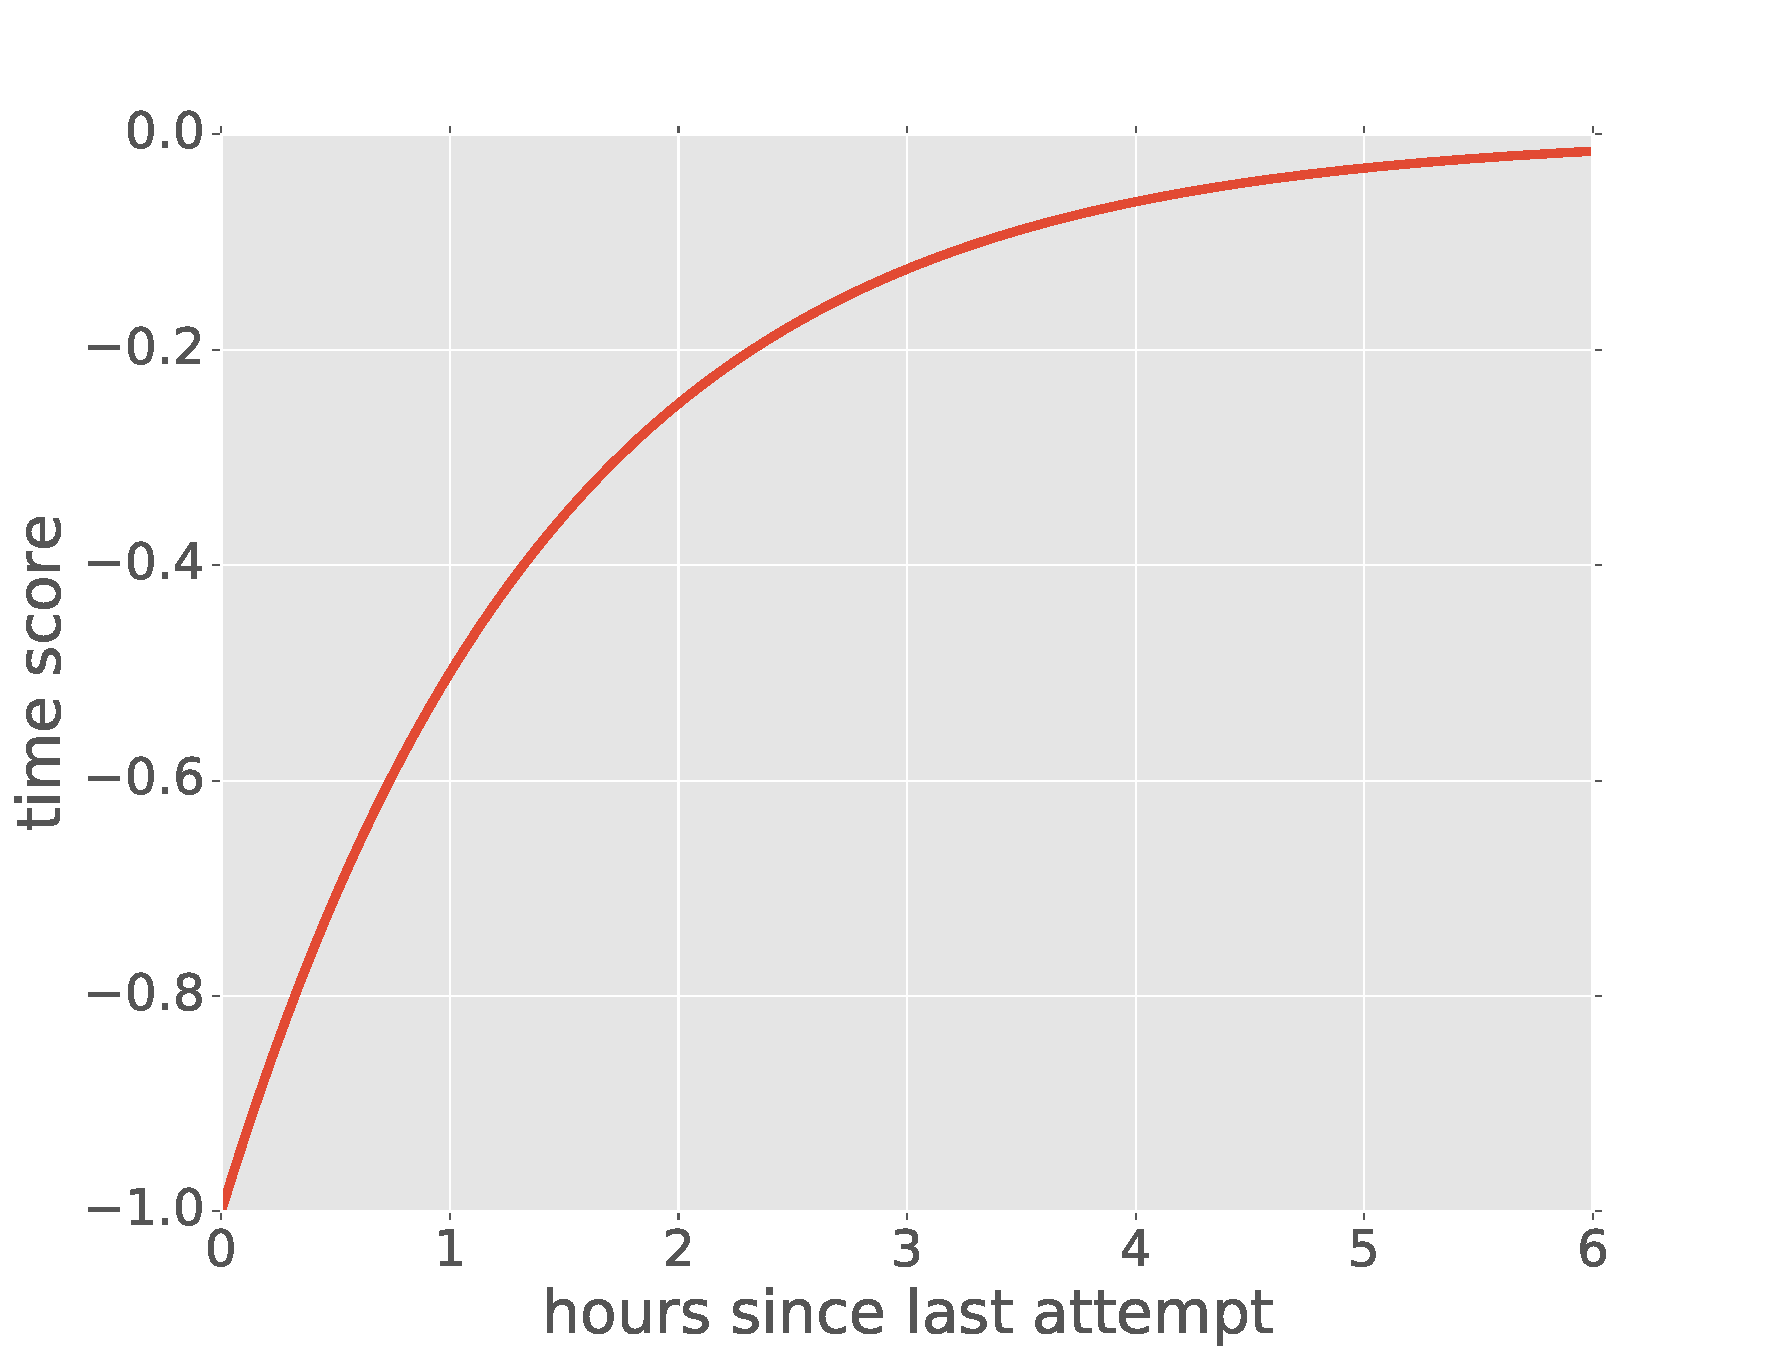
\includegraphics[height=4cm]{img/score-time.pdf}
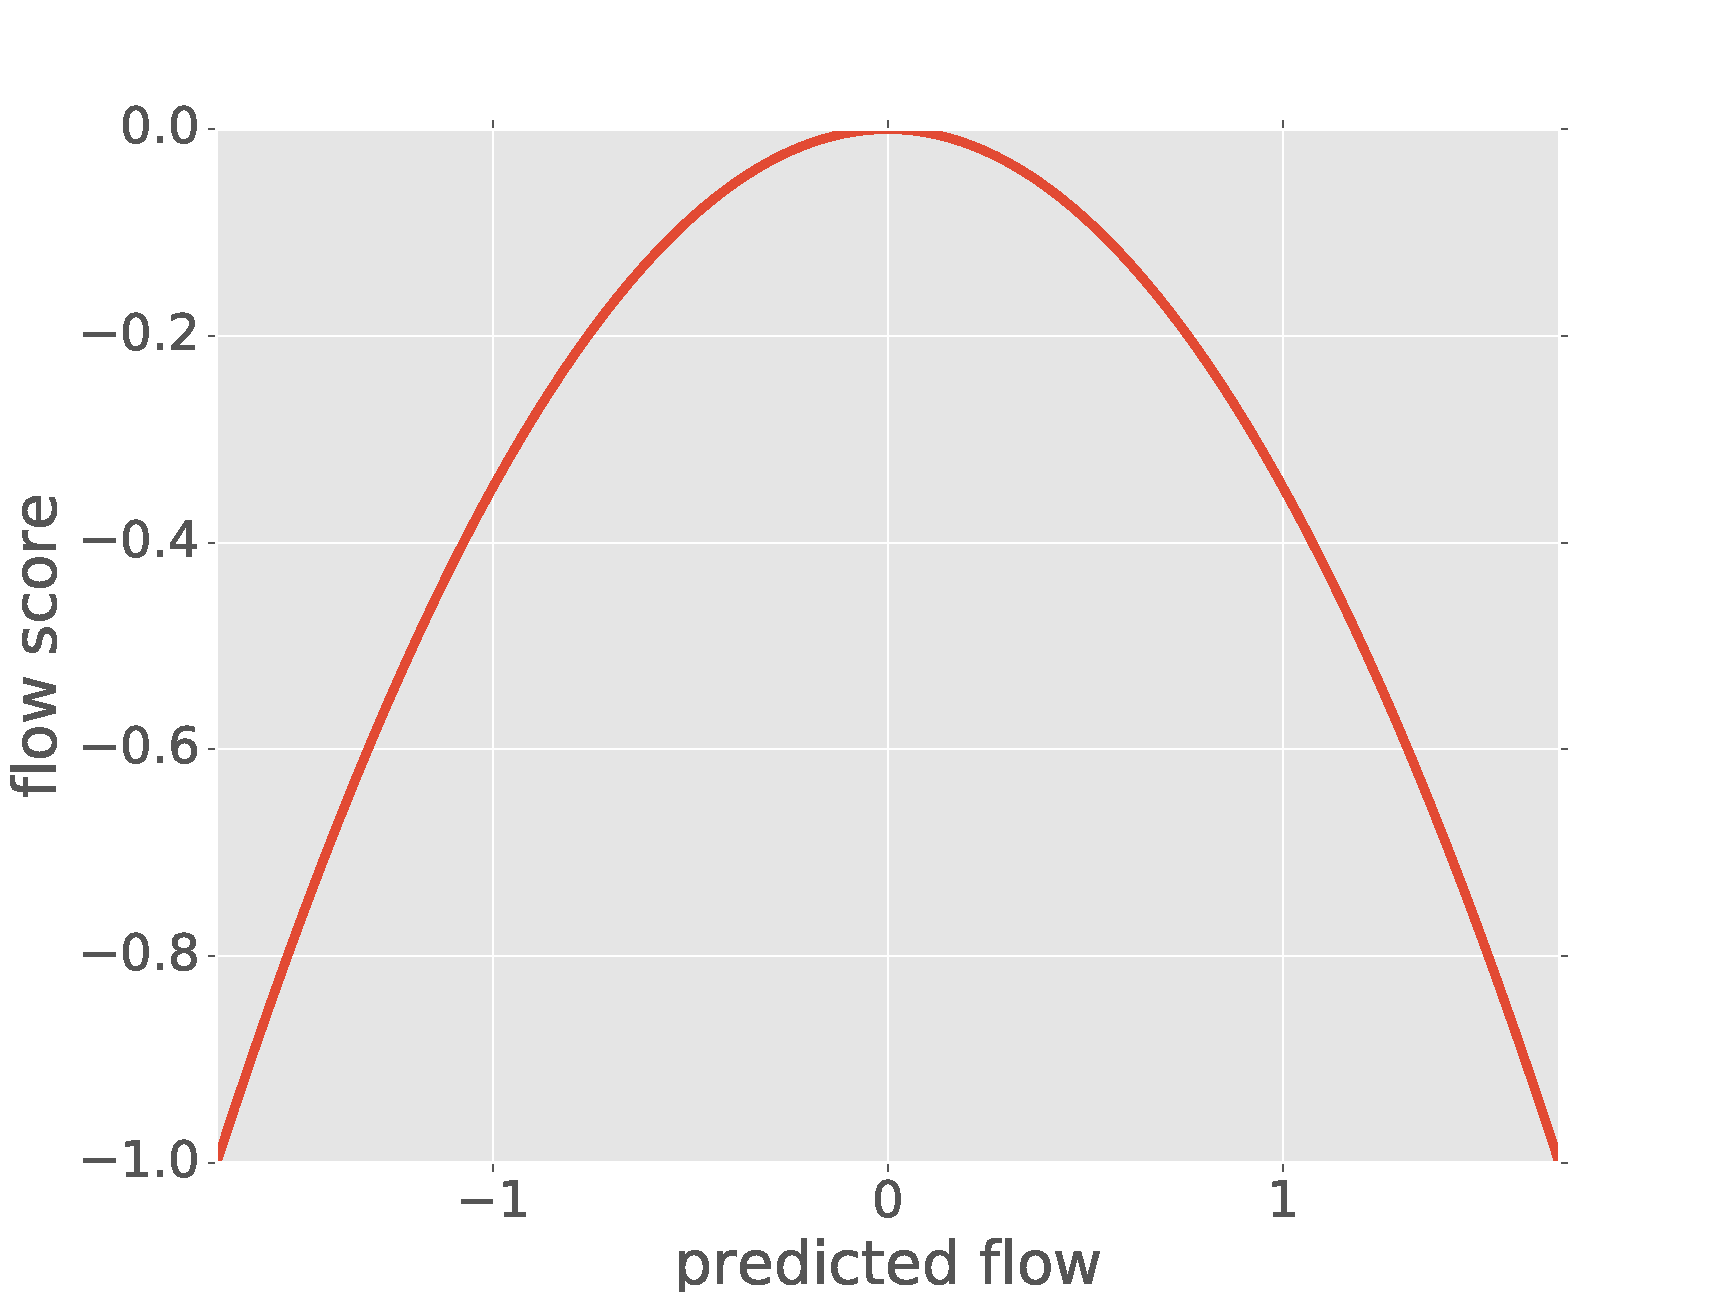
\includegraphics[height=4cm]{img/score-flow.pdf}
\end{frame}

\begin{frame}
\frametitle{Initial student skill}
\begin{itemize}
\item assuming low initial skill
\item $\beta_s = -1$
\item $\alpha_s = (-1, -1, -1, -1, -1, -1)$
\end{itemize}
\end{frame}

\begin{frame}
\frametitle{Initial task difficulty}
\begin{itemize}
\item content based approach
\item difficulty bias: magic formula
  \begin{itemize}
  \item based on number of concepts, number of blocks, maze size, number of free fields, number of tokens and block limit
  \end{itemize}
\item factors: $0.2$ if contains the factor, else $0$
\end{itemize}
\end{frame}

%\begin{frame}
%\frametitle{Initial tasks difficulty}
%\small
%\begin{equation*}
%\begin{split}
%  \mbox{diff}(t) = & \tanh ((b_t - K_1) + (5 m - K_2) + (5 l_t - K_3) \\
%                   & + 0.5\ln{(f)}) / K_{13}) \\
%                   & + K_8 (c_t - K_8)
%\end{split}
%\end{equation*}
%\end{frame}


\begin{frame}
\frametitle{Parameters update}
\begin{itemize}
\item student bias update
  \begin{itemize}
  \item report: $\beta_s \leftarrow \beta_s - K_r(\hat{f}_{st} - f_{st})$
  \item learning: $\beta_s \leftarrow \beta_s + K_{l} e^{- K_{j} \beta_s}$
  \end{itemize}
\item skill factors update
  \begin{itemize}
  \item only for factors in tasks ($a_t[i] > 0$)
  \item $\alpha_s[i] \leftarrow \max(\alpha_s[i], f_{st})$
  \end{itemize}
\item task bias update
  \begin{itemize}
  \item $b_s \leftarrow b_s + \frac{K_t}{n + K_n}(\hat{f}_{st} - f_{st})$
  \item $n$ -- updates count
  \end{itemize}
\item task factors -- fixed
\end{itemize}
\end{frame}

\begin{frame}
\frametitle{Simulation}
\imageH{practice-simulation-normal.pdf}
\end{frame}

\begin{frame}
\frametitle{Simulation -- stupid}
\imageH{practice-simulation-stupid.pdf}
\end{frame}

\begin{frame}
\frametitle{Simulation -- genius}
\imageH{practice-simulation-genius.pdf}
\end{frame}

\begin{frame}
\frametitle{Evaluation}
\begin{itemize}
\item not enough data
\end{itemize}
TODO: (at least we can show some basic statistics and how the task difficulties changed in time)
\end{frame}

\begin{frame}
\frametitle{Experience report}
\begin{itemize}
\item difficulty is changing
\item clear task instructions
\item non-intuitive user interface
\end{itemize}
\end{frame}

\begin{frame}
\frametitle{Implementation}
\begin{itemize}
\item core: Python 3.5
\item backend: Django, layered architecture
\item frontend: AngularJS (modularity, promises), Blockly, JS-interpreter, Bootstrap
\item analysis: pandas, matplotlib
\item infrastructure: Git, GitHub, Virtualenv, pip, make, Django, Grunt, Bower, Karma
\item deployment: Nginx, Gunicorn, PostgreSQL
\item 45 unit tests, 195 commits, 44 closed issues
\end{itemize}
\end{frame}


\begin{frame}
\frametitle{Summary}
\begin{itemize}
\item system for adaptive learning of programming
\item Blockly language, tasks in a maze
\item flow, Elo model, factors
\item first prototype: \url{http://flocs.thran.cz}
\item repo: \url{https://github.com/effa/flocs}
\end{itemize}
\end{frame}

\end{document}
